%; whizzy paragraph -pdf xpdf -latex ./whizzypdfptex.sh
%; whizzy-paragraph "^\\\\begin{frame}\\|\\\\emtext"
% latex beamer presentation.
% platex, latex-beamer でコンパイルすることを想定。 

%     Tokyo Debian Meeting resources
%     Copyright (C) 2012 Junichi Uekawa

%     This program is free software; you can redistribute it and/or modify
%     it under the terms of the GNU General Public License as published by
%     the Free Software Foundation; either version 2 of the License, or
%     (at your option) any later version.

%     This program is distributed in the hope that it will be useful,
%     but WITHOUT ANY WARRANTY; without even the implied warreanty of
%     MERCHANTABILITY or FITNESS FOR A PARTICULAR PURPOSE.  See the
%     GNU General Public License for more details.

%     You should have received a copy of the GNU General Public License
%     along with this program; if not, write to the Free Software
%     Foundation, Inc., 51 Franklin St, Fifth Floor, Boston, MA  02110-1301 USA

\documentclass[cjk,dvipdfmx,12pt]{beamer}
\usetheme{Tokyo}
\usepackage{monthlypresentation}

%  preview (shell-command (concat "evince " (replace-regexp-in-string "tex$" "pdf"(buffer-file-name)) "&")) 
%  presentation (shell-command (concat "xpdf -fullscreen " (replace-regexp-in-string "tex$" "pdf"(buffer-file-name)) "&"))
%  presentation (shell-command (concat "evince " (replace-regexp-in-string "tex$" "pdf"(buffer-file-name)) "&"))

%http://www.naney.org/diki/dk/hyperref.html
%日本語EUC系環境の時
\AtBeginDvi{\special{pdf:tounicode EUC-UCS2}}
%シフトJIS系環境の時
%\AtBeginDvi{\special{pdf:tounicode 90ms-RKSJ-UCS2}}

\title{東京エリアDebian勉強会}
\subtitle{第93回 2012年10月度}
\author{上川純一\\dancer@debian.org}
\date{2012年10月20日}
\logo{
\includegraphics[width=8cm]{image200607/openlogo-light.eps}}

\begin{document}

\frame{\titlepage{}}

\begin{frame}{設営準備にご協力ください。}
会場設営よろしくおねがいします。
\end{frame}

\begin{frame}{Agenda}
\begin{minipage}[t]{0.45\hsize}
  \begin{itemize}
  \item 注意事項
	\begin{itemize}
	 \item 飲食禁止
	 \item 宗教禁止
	 \item 営利活動禁止
	\end{itemize}
   \item 最近あったDebian関連のイベント報告
	\begin{itemize}
        \item 第91回 東京エリアDebian勉強会
        \item 第0回Debianパッケージング道場
	\end{itemize}
   \item DWN quiz
   \item 事前課題紹介
 \end{itemize}
\end{minipage} 
\begin{minipage}[t]{0.45\hsize}
 \begin{itemize}
  \item Haskell の Debian packaging 周辺について語ります
  \item レゴでなめこ収穫期
  \item xf86-input-mtrack

 \end{itemize}
\end{minipage}
\end{frame}


\section{DWN quiz}
\emtext{DWN quiz}
\begin{frame}{Debian 常識クイズ}

Debian の常識、もちろん知ってますよね?
知らないなんて恥ずかしくて、知らないとは言えないあんなことやこんなこと、
みんなで確認してみましょう。

今回の出題範囲は\url{debian-devel-announce@lists.debian.org},
\url{debian-devel@lists.debian.org} に投稿された
内容とDebian Project Newsなどからです。

\end{frame}

\subsection{問題}
%; whizzy-master ../debianmeetingresume201210.tex
% 以上の設定をしているため、このファイルで M-x whizzytex すると、whizzytexが利用できます。
%

\santaku
{9/29 に行われた Debian 6.0 のアップデートは何回目でしょうか。}
{5}
{6}
{7}
{B}
{6.0.6 です。}

\santaku
{DMUA フィールドがなくなり、Debian Maintainerのアップロードが変更されます。今後、アップロードの際にどのように作業する必要があるか?}
{FTP masterに電話}
{スポンサーに dak の処理を依頼する}
{専用アップローダにアップロード}
{B}
{}

\santaku
{IRC 経由でVCS リポジトリを監視するサービスで終了したものは?}
{ICPO}
{NPA}
{CIA}
{C}
{KGBに移行。ICPA:  International Criminal Police Organization, NAP:National Police Agency, CIA: Central Intelligence Agency}

\santaku
{Debian Policy メンテナに新しく入ったのは誰か?}
{Kei Hibino}
{Colin Watson}
{Charles Plessy}
{C}
{Andrew McMillan, Colin Watson, Manoj Srivastava が抜けた}

\santaku
{Checksums-SHA1,SHA256 の取り扱いが変更になったが、どう変更されたか?}
{今まで無視されていました。ごめんね。}
{オプションだったので、必須としました。}
{これらは廃止し、SHA-512のみにします。}
{B}
{Bug\#690293}



\emtext{事前課題}
{\footnotesize
 

\begin{prework}{ $B4d>>(B $B?.MN(B }

(1) erlang $B$H(BHaskell $B$r>/!9!#(B

(2) Real World Haskell$B!#%W%m%0%i%_%s%0(BErlang$B!#(B

(3) Erlang $B$N(B $B%S%k%I%7%9%F%`$G$"$k(B rebar $B$r$b$&$A$g$C$HM}2r$7$?$$!#(B


\end{prework}

\begin{prework}{ yamamoto }

(1) $B4X?t7?%W%m%0%i%_%s%08@8l$NMxMQ7P83(B $B!](B $B$J$7(B
(2) $B$*4+$a=q@R(B $B!](B $BFI$s$@$3$H!"$"$j$^$;$s(B
(3) $B;H$C$F$_$?$$%=%U%H(B $B!](B $BFC$K$J$7(B

$B$G$b!"(Bhaskell $B$O$J$s$+LLGr$=$&$@$7!"3X$s$G$_$h$&$+$J!)$H$+9M$($F$$$^$9!#(B
\end{prework}

\begin{prework}{ alice.ferrazzi }


\end{prework}

\begin{prework}{ $BNkLZ?rJ8(B }

(1)Debian $B$G$N4X?t7?%W%m%0%i%_%s%08@8l$NMxMQ7P83$H$=$N;~$K46$8$?;vJA!J(BLisp, Emacs Lisp, OCaml, Haskell $BEy!K(B
Erlang $B!&!&!&$5$o$jDxEY$G$9$,!"(BRiak$B$J$I$N<BMQ%l%Y%k$N%=%U%H%&%'%"$G;HMQ$5$l$F$$$kE@$d!"J,;64D6-$dL5Dd;_$K8@8l%l%Y%k$GBP1~$5$l$F$$$kE@$,LLGr$+$C$?$G$9!#(BRiak$B$+$i>pJs$r<h$C$?$jF~$l$?$j$9$k$@$1$J$i$PHf3SE*4JC1$KA`:n$G$-$^$7$?!#(B
Haskell $B!&!&!&$5$o$jDxEY$G$9$,!"(BHaskell$B9%$-$J?M$,B?$$$?$a3X$V$K$ONI$$8@8l$@$H46$8$^$7$?!#(B

(2) $B4X?t7?%W%m%0%i%_%s%08@8l=i?4<T$K8~$1$?$*4+$a=q@R$H$=$N%&%j$N>R2p(B
Erlang$B$O$J$+$J$+K\$,$J$+$C$?$G$9!#(BHaskell$B$O!V$9$4$$(BHaskell$B$?$N$7$/3X$\$&!*!W$,FI$_$d$9$$$h$&$K46$8$^$9$,!"$^$@M}2r$G$-$F$^$;$s!#(B

(3) $B4X?t7?8@8l$G<BAu$5$l$F$$$k!";H$C$F$_$?$$%=%U%H$r$"$2$F$/$@$5$$(B
Riak
xmonad

\end{prework}

\begin{prework}{ $B5HLn(B(yy\_y\_ja\_jp) }

(1) $B:G6a(BHaskell$B$r?($C$F$$$^$9!%(Bcabal-debian$B$r$b$&>/$7CN$j$?$$$G$9!%(B
\end{prework}

\begin{prework}{ $B%-%?%O%i(B }

(1) Haskell $BF~Lg=q$N%5%s%W%k$rF0$+$7$?DxEY!"(B
    apt-get$B$G4JC1$KF3F~$G$-$F46F0$7$?$h$&$J5-21$,!&!&!&!#(B
(2) Haskell$B$NF~Lg=q$r(B2$B:}$[$IFI$_$^$7$?$,!"6&$K(Bmonad$B$G(B
    $B:C@^$7$?!":G6a$NK\$OFI$s$G$$$J$$!#(B
(3) $BFC$K$J$7!#(B

\end{prework}

\begin{prework}{ dictoss($B?yK\!!E5=<(B) }

(1) emacs.el$B$r=q$/$/$i$$$G$J$s$H$J$/;H$C$F$$$k46$8$G$9!#%7%s%0%k%/%)!<%F!<%7%g%s$OJD$8$J$/$F$$$$>l9g$,$"$k$N$G$=$l$K8MOG$&$3$H$,$"$j$^$9!#(B
\end{prework}

\begin{prework}{ $BLn<s(B }

elisp$B$G$A$g$C$H(Bmajor mode$B$H(Bshinbum module$B$r=q$$$F$_$?$3$H$,$"$k$0$i$$$G$9!#(B
$B4X?t7?%W%m%0%i%_%s%0$H$$$&%l%Y%k$K;j$j$^$;$s$G$7$?!#(B

\end{prework}

\begin{prework}{ @Lost\_dog\_ }

 (1) Haskell:$B7?0BA4$N$"$j$,$?$_$,J,$+$C$?(B
 (2) $B!X$9$4$$(BHaskell$B$?$N$7$/3X$\$&(B!$B!Y$O4X?t7?$NJ70O5$$rPmbW$G$-$k!#K\5$$GJY6/$9$k$J$i!"$b$C$H2&F;$N%F%-%9%H$rA*$s$@$[$&$,$h$$$+$b!#(B
 (3) yi-editor
\end{prework}

\begin{prework}{ $BF|HfLn(B $B7<(B }

(1) Haskell, OCaml $B$H$b$K(B Debian $B$K$OB??t$N%Q%C%1!<%8$,$"$C$F$9$P$i$7$$$G$9!#(B

(2)
\begin{itemize}
\item {\bf $B%W%m%0%i%_%s%0(BHaskell\\ - Graham Hutton ($BCx(B), $B;3K\(B $BOBI'(B ($BK]Lu(B)]}\\
$B:G=i$KFI$`$J$i$3$l$G$9!#4X?t%W%m%0%i%_%s%0$N%H%T%C%/$rJ?0W$K2r@b$7$J$i$,(BHaskell$B$r;n$7$F$$$-$^$9!#(B
\item {\bf $B$9$4$$(BHaskell$B$?$N$7$/3X$\$&(B!\\ - Miran Lipovaa ($BCx(B), $BEDCf(B $B1Q9T(B ($BK]Lu(B), $BB<<g(B $B?r9T(B ($BK]Lu(B)}\\
$B!V%W%m%0%i%_%s%0(BHaskell$B!W$N<!$O$3$l$@$H;W$$$^$9!#$h$jJ#;($J7?$N5!G=$r$b4^$a$F(BHaskell$B$N2r@b$,?J$s$G$$$-$^$9!#(B
\item {\bf Real World Haskell $B<B@o$G3X$V4X?t7?8@8l%W%m%0%i%_%s%0(B\\
 - Bryan O'Sullivan ($BCx(B), John Goerzen ($BCx(B), Don Stewart ($BCx(B), $B;32<(B $B?-IW(B ($BK]Lu(B), $B0KEl(B $B>!Mx(B ($BK]Lu(B), $B3t<02q<R%?%$%`%$%s%?!<%a%G%#%"(B ($BK]Lu(B)}\\
$B<B:]$K(BHaskell$B$r8=>l$GMxMQ$7$F$k?M$?$A$,=q$$$?K\$H$7$F$N2ACM$,$"$kK\$G$9!#(B
Haskell$B$K$b$$$m$$$m$J%i%$%V%i%j$,$"$j!"$=$NMxMQNc$H$7$F;29M$K$J$k$H;W$$$^$9!#(B
$B>/$78E$$$N$,LdBjE@$G$9!#(B
\end{itemize}

(3) OCaml$B$G:n$i$l$F$$$kDjM}>ZL@4o(BCoq$B$r$&$^$/;H$($k$h$&$K$J$j$?$$$G$9!#$"$H(BHaskell$B$G$$$m$$$m:n$kB&$K$^$o$j$?$$!#(B

\end{prework}

}

\emtext{xf86-input-mtrack}

\begin{frame}{xf86-input-mtrack}

\begin{itemize}
\item 昔の Macbook \\
pre-multitouchサポート
\item 最近の Macbook Pro / Air /Magic Trackpad\\
マルチタッチサポート。\\
最初は synaptics ドライバでは動作しませんでした。\\
xserver-xorg-input-mrack / multitouch を使う必要があります。
\end{itemize}

\end{frame}


\begin{frame}{synaptics と mtrack}
\begin{itemize}
\item synaptics では、プロトコルA のみのサポート(だった?)\\
これはタッチIDを持っていないため、トラッキングコンタクトを管理できません。
%ステートレス
%ステートフル

\item mtrack では、タッチIDをサポートしたプロトコルB をサポート。
これにより、より細かいタッチパッドの制御ができるようになっています。

\item Macbook Pro等に搭載されている BCM5974 の機能をサポートしています。\\
\end{itemize}

\end{frame}

\begin{frame}

\begin{itemize}
\item また、「プロトコルB」をLinuxカーネルから受信し、それをXドライバにわかりやすい
(人間にとってわかりやすい)形にデータを形成するライブラリ mtdev を
使います。
\end{itemize}
\begin{center}
\includegraphics[width=0.5\hsize]{image201210/mtrack.eps}
\end{center}

\end{frame}

\begin{frame}[containsverbatim]

プロトコルA
\begin{minipage}[t]{0.4\hsize}
\begin{commandline}
ABS_MT_POSITION_X x[0]
ABS_MT_POSITION_Y y[0]
SYN_MT_REPORT
ABS_MT_POSITION_X x[1]
ABS_MT_POSITION_Y y[1]
SYN_MT_REPORT
SYN_REPORT
\end{commandline}
\end{minipage}

プロトコルB
\begin{minipage}[t]{0.4\hsize}
\begin{commandline}
ABS_MT_SLOT 0
ABS_MT_TRACKING_ID 45
ABS_MT_POSITION_X x[0]
ABS_MT_POSITION_Y y[0]
ABS_MT_SLOT 1
ABS_MT_TRACKING_ID 46
ABS_MT_POSITION_X x[1]
ABS_MT_POSITION_Y y[1]
SYN_REPORT
\end{commandline}
\end{minipage}

\end{frame}

\begin{frame}{multitouch と mtrack}

\begin{itemize}
\item multitouch\\
基本的な設定
\item mtrack\\
multitouch からのフォーク。\\
細かい機能のサポート。\\
\end{itemize}

\end{frame}

\begin{frame}[containsverbatim]{Debian で使う}

\begin{itemize}
\item Debian では既にパッケージ化されており、APT でインストールできます。

\begin{commandline}
$ sudo apt-get install xserver-xorg-input-mtrack
\end{commandline}
%$
\end{itemize}

\end{frame}

\begin{frame}[containsverbatim]{デフォルトの設定}

\begin{commandline}
Section "InputClass"
    MatchIsTouchpad "true"
    Identifier "Multitouch Touchpad"
    Driver "mtrack"
EndSection
\end{commandline} 

\end{frame}

\begin{frame}[containsverbatim]
インストールした段階では、デフォルトの設定で動作します。
細かい設定を行うために多くの項目があります。
\begin{table}[htb]
  \begin{tabular}{llc}
    項目 & 内容 & デフォルト値 \\
    TrackpadDisable & トラックパッド機能の動作内容と無効化 & 0 \\
    Sensitivity & トラックパッドのスピード & 1 \\
    FingerHigh & 指がタッチとして検知される圧力 & 5 \\
    FingerLow & 指がリリースとして検知される圧力 & 5 \\
    IgnoreThumb & 親指であるとわかるタッチを無視するか & False \\
    IgnorePalm & 手の平であるとわかるタッチを無視するか & False \\
    DisableOnThumb & 親指がさわっているとき全てのトラックパッドを無効にするか & False \\
    DisableOnPalm & 手の平ががさわっているとき全てのトラックパッドを無効にするか & False \\
    ThumbRatio & 親指の幅/長比率 & 70 \\
    ThumbSize & 親指の最小限のサイズ & 25 \\
    PalmSize & 手の平の最小限のサイズ & 10 \\
  \end{tabular}
\end{table}
.......

\end{frame}

\begin{frame}[containsverbatim]{有効な設定}

トラックパッドのシングルタップを無効にする\\
トラックパッドに触っても(シングルタップしても)何も起きなくなります。

\begin{commandline}
Option "TapButton1" "0"
Option "TapButton2" "0"
Option "TapButton3" "0"
\end{commandline}

\end{frame}

\begin{frame}[containsverbatim]{有効な設定}

2本指スクロールの動きををOS Xと同じにする
\begin{commandline}
Option "ScrollUpButton" "5"
Option "ScrollDownButton" "4"
\end{commandline}

\end{frame}

\begin{frame}[containsverbatim]{その他の情報}

\begin{itemize}

\item 現在の mtrack ドライバは synaptics のように設定値を動的に変更できません。

\item これでは細かい設定等を行う時に大変なので常に設定を変更できるようにするためのパッチを
作成し、アップストリームに送りました。
\url{https://github.com/BlueDragonX/xf86-input-mtrack/pull/41}

パッチを適用し、以下の設定を行なってXサーバを立ち上げると
動的に設定を変更できるようになります。
\begin{commandline}
Option "SHMConfig" "true"
\end{commandline}

\end{itemize}

\end{frame}

\begin{frame}{設定ツール}

肝心の設定用のツールですが、適当に作ったので後日公開します。

\end{frame}

\begin{frame}{デモ}

\end{frame}

\begin{frame}{Debianでマルチタッチを使う場合にはどうしたらいいのか}

\begin{itemize}
\item 大統一Debian勉強会での赤部さんの発表\footnote{\url{http://gum.debian.or.jp/download/debian-gum-presentation.akabe.pdf}}
にもあったように、Debian ではまだマルチタッチを
提供するツール等が十分ではありません。

\item X や GTK+ などでは既にマルチタッチは対応していますが、
それを使うアプリケーションがなく、Ubuntu で採用されている utouch \footnote{\url{https://wiki.ubuntu.com/Multitouch}}
関連のライブラリもまだパッケージになっていない状態です(ITPはされています)。
\item よって Debian ではまだ iPad や Android タブレット相当の操作はできないと思われます。

\end{itemize}

\end{frame}

\begin{frame}{まとめ}

\begin{itemize}
\item mtrack ドライバでマルチタッチの制御はできるようになっていますが、アプリケーションが
追いついていないのが現状です。
\item ユニバーサルオペレーティングシステムを目指す以上、マルチタッチは避けて通れない機能なので早くサポートされてほしいものです。
\end{itemize}

\end{frame}







\section{今後のイベント}
\emtext{今後のイベント}
\begin{frame}{今後のイベント}
\begin{itemize}
 \item 2012年/11月 Debian勉強会 \\
BSP やるらしいですが?
\end{itemize}
\end{frame}

\section{今日の宴会場所}
\emtext{今日の宴会場所}
\begin{frame}{今日の宴会場所}
未定
\end{frame}

\end{document}

;;; Local Variables: ***
;;; outline-regexp: "\\([ 	]*\\\\\\(documentstyle\\|documentclass\\|emtext\\|section\\|begin{frame}\\)\\*?[ 	]*[[{]\\|[]+\\)" ***
;;; End: ***
